\documentclass[tikz,border=8pt]{standalone}
\usepackage{amsmath,amssymb}
\usetikzlibrary{arrows.meta,automata,positioning,quotes}
\begin{document}
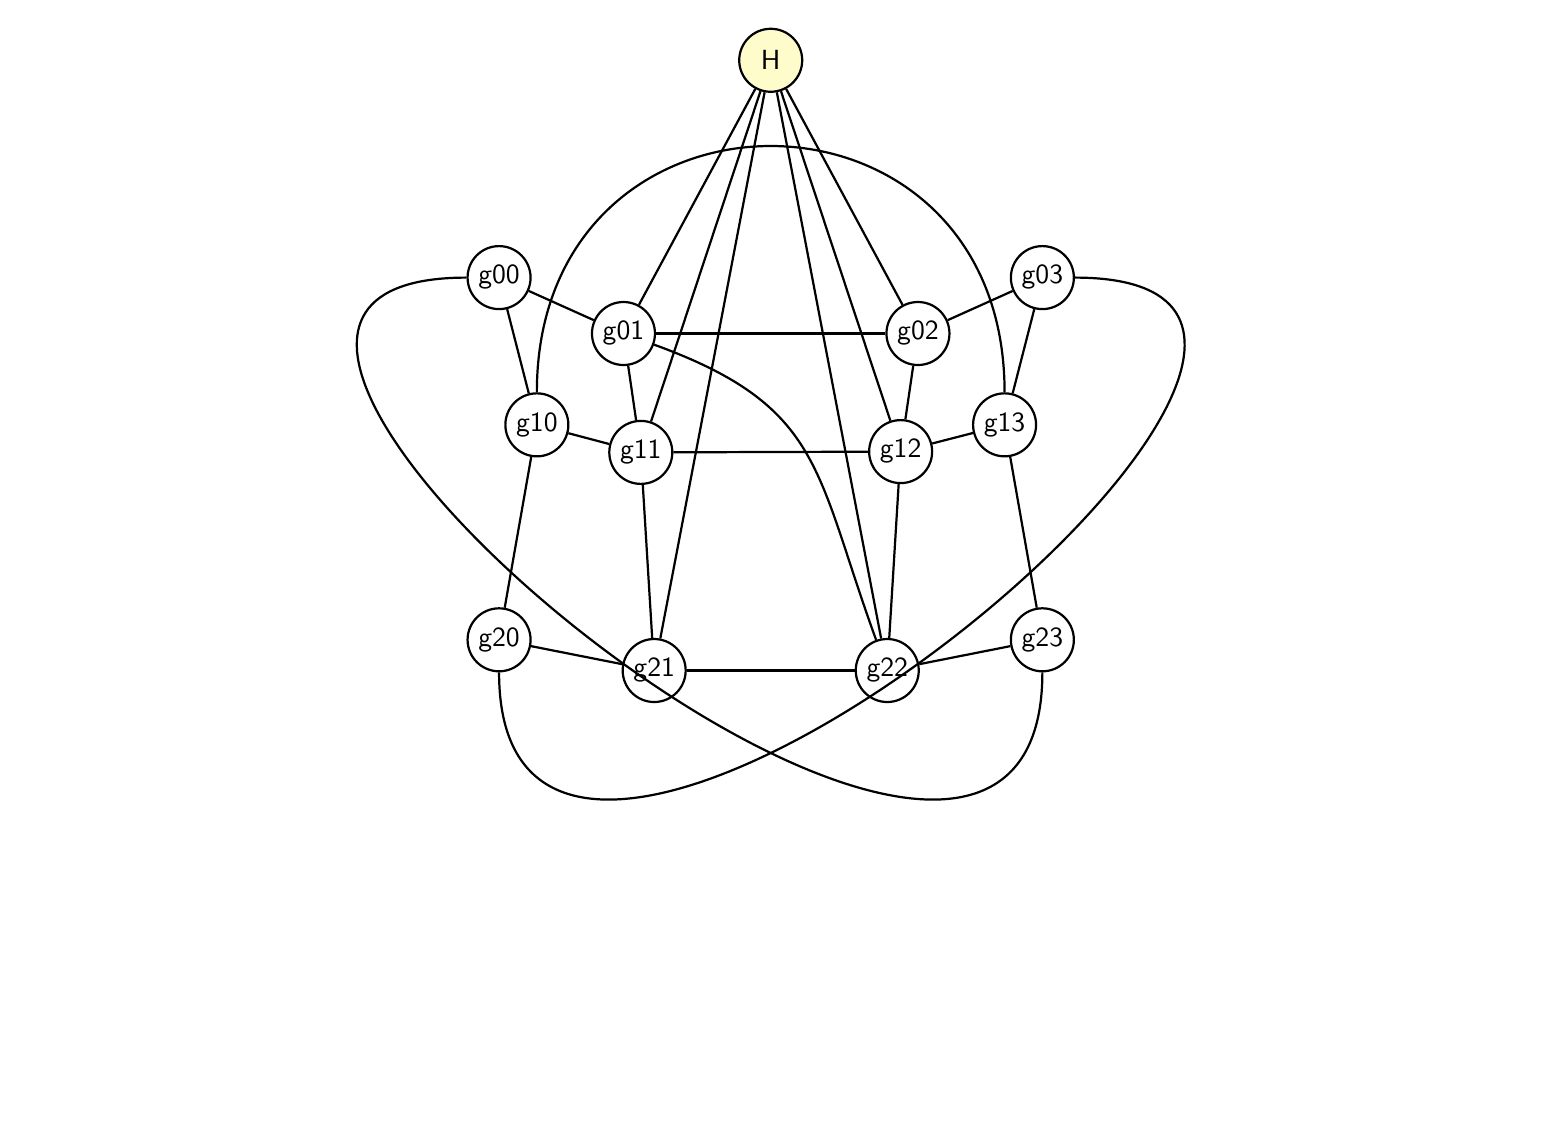
\begin{tikzpicture}[x=1cm,y=1cm]
\tikzset{
  graphnode/.style={circle,draw,thick,minimum size=8mm,inner sep=1pt,font=\sffamily},
  directed/.style={-{Stealth[length=2.4mm]},thick},
  undirected/.style={thick}
}
\node[graphnode] (n_g00) at (-0.45,0.25) {g00};
\node[graphnode] (n_g01) at (1.13,-0.46) {g01};
\node[graphnode] (n_g02) at (4.87,-0.46) {g02};
\node[graphnode] (n_g03) at (6.45,0.25) {g03};
\node[graphnode] (n_g10) at (0.03,-1.62) {g10};
\node[graphnode] (n_g11) at (1.35,-1.97) {g11};
\node[graphnode] (n_g12) at (4.65,-1.96) {g12};
\node[graphnode] (n_g13) at (5.97,-1.62) {g13};
\node[graphnode] (n_g20) at (-0.45,-4.35) {g20};
\node[graphnode] (n_g21) at (1.52,-4.74) {g21};
\node[graphnode] (n_g22) at (4.48,-4.74) {g22};
\node[graphnode] (n_g23) at (6.45,-4.35) {g23};
\node[graphnode,fill=yellow!20] (n_H) at (3.00,3.01) {H};
\draw[undirected] (n_g00) -- (n_g01);
\draw[undirected] (n_g01) -- (n_g02);
\draw[undirected] (n_g02) -- (n_g03);
\draw[undirected] (n_g10) -- (n_g11);
\draw[undirected] (n_g11) -- (n_g12);
\draw[undirected] (n_g12) -- (n_g13);
\draw[undirected] (n_g20) -- (n_g21);
\draw[undirected] (n_g21) -- (n_g22);
\draw[undirected] (n_g22) -- (n_g23);
\draw[undirected] (n_g00) -- (n_g10);
\draw[undirected] (n_g10) -- (n_g20);
\draw[undirected] (n_g01) -- (n_g11);
\draw[undirected] (n_g11) -- (n_g21);
\draw[undirected] (n_g02) -- (n_g12);
\draw[undirected] (n_g12) -- (n_g22);
\draw[undirected] (n_g03) -- (n_g13);
\draw[undirected] (n_g13) -- (n_g23);
\draw[undirected] (n_H) -- (n_g01);
\draw[undirected] (n_H) -- (n_g02);
\draw[undirected] (n_H) -- (n_g11);
\draw[undirected] (n_H) -- (n_g12);
\draw[undirected] (n_H) -- (n_g21);
\draw[undirected] (n_H) -- (n_g22);
\draw[undirected] (n_g00) to[out=180,in=-90,looseness=1.6] (n_g23);
\draw[undirected] (n_g03) to[out=0,in=-90,looseness=1.6] (n_g20);
\draw[undirected] (n_g10) to[out=90,in=90,looseness=1.8] (n_g13);
\draw[undirected] (n_g01) to[out=-20,in=110,looseness=1.25] (n_g22);
\end{tikzpicture}
\end{document}
